\documentclass[tikz,border=8pt]{standalone}
\usetikzlibrary{arrows.meta,positioning,calc,fit}

\begin{document}
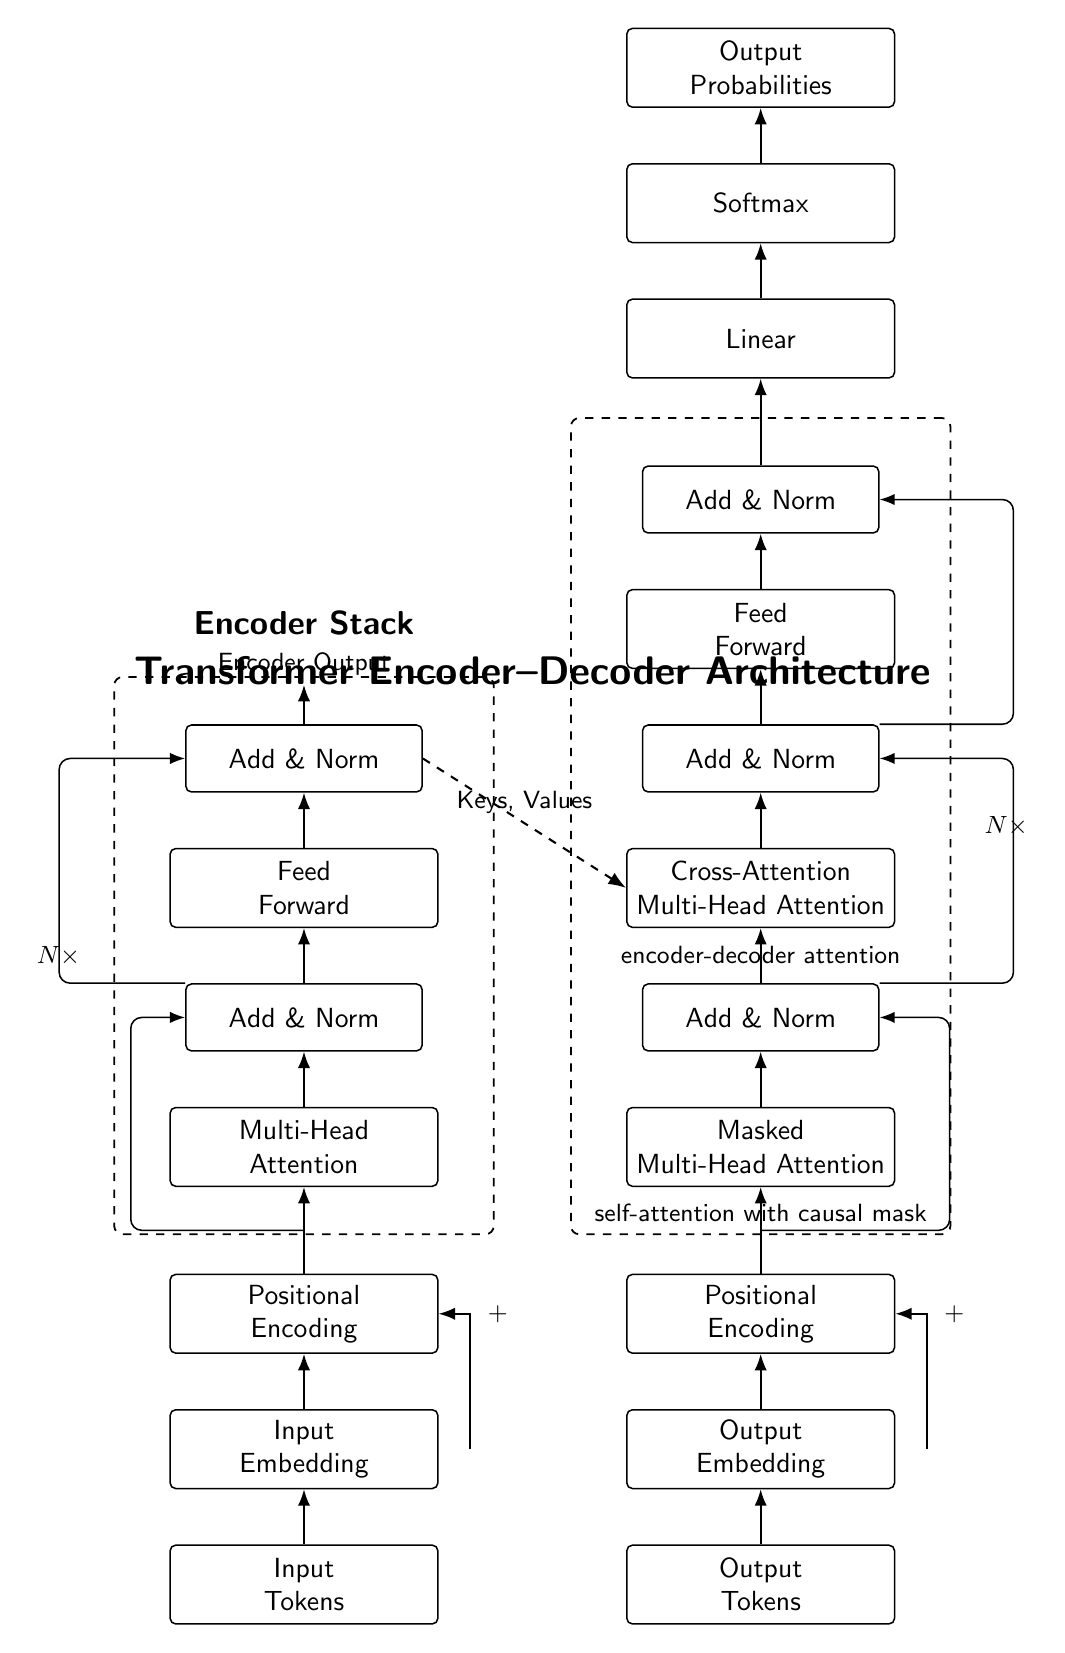
\begin{tikzpicture}[
  font=\sffamily,
  >=Latex,
  node distance=7mm,
  block/.style={
    draw,
    rounded corners=2pt,
    minimum width=34mm,
    minimum height=10mm,
    align=center,
    fill=white,
    line width=0.55pt
  },
  smallblock/.style={
    draw,
    rounded corners=2pt,
    minimum width=30mm,
    minimum height=8.5mm,
    align=center,
    fill=white,
    line width=0.55pt
  },
  stackbox/.style={
    draw,
    rounded corners=3pt,
    dashed,
    inner xsep=7mm,
    inner ysep=6mm,
    line width=0.65pt
  },
  arrow/.style={->, line width=0.65pt},
  residual/.style={->, line width=0.55pt, rounded corners=4pt},
  cross/.style={->, line width=0.75pt, dashed},
  label/.style={font=\sffamily\small},
  title/.style={font=\sffamily\bfseries\large}
]

% Encoder bottom
\node[block] (src) at (0,0) {Input\\Tokens};
\node[block, above=of src] (srcemb) {Input\\Embedding};
\node[block, above=of srcemb] (srcpos) {Positional\\Encoding};

% Encoder stack
\node[block, above=11mm of srcpos] (encmha) {Multi-Head\\Attention};
\node[smallblock, above=of encmha] (encadd1) {Add \& Norm};
\node[block, above=of encadd1] (encffn) {Feed\\Forward};
\node[smallblock, above=of encffn] (encadd2) {Add \& Norm};
\node[above=5mm of encadd2, label] (encoutlabel) {Encoder Output};

\node[stackbox, fit=(encmha)(encadd1)(encffn)(encadd2)] (encstack) {};
\node[title, above=4mm of encstack] {Encoder Stack};
\node[label, left=3mm of encstack] {$N\times$};

% Decoder bottom
\node[block] (tgt) at (58mm,0) {Output\\Tokens};
\node[block, above=of tgt] (tgtemb) {Output\\Embedding};
\node[block, above=of tgtemb] (tgtpos) {Positional\\Encoding};

% Decoder stack
\node[block, above=11mm of tgtpos] (decmask) {Masked\\Multi-Head Attention};
\node[smallblock, above=of decmask] (decadd1) {Add \& Norm};
\node[block, above=of decadd1] (deccross) {Cross-Attention\\Multi-Head Attention};
\node[smallblock, above=of deccross] (decadd2) {Add \& Norm};
\node[block, above=of decadd2] (decffn) {Feed\\Forward};
\node[smallblock, above=of decffn] (decadd3) {Add \& Norm};

\node[stackbox, fit=(decmask)(decadd1)(deccross)(decadd2)(decffn)(decadd3)] (decstack) {};
\node[title, above=4mm of decstack] {Decoder Stack};
\node[label, right=3mm of decstack] {$N\times$};

% Output head
\node[block, above=11mm of decadd3] (linear) {Linear};
\node[block, above=of linear] (softmax) {Softmax};
\node[block, above=of softmax] (prob) {Output\\Probabilities};

% Main encoder arrows
\draw[arrow] (src) -- (srcemb);
\draw[arrow] (srcemb) -- (srcpos);
\draw[arrow] (srcpos) -- (encmha);
\draw[arrow] (encmha) -- (encadd1);
\draw[arrow] (encadd1) -- (encffn);
\draw[arrow] (encffn) -- (encadd2);
\draw[arrow] (encadd2) -- (encoutlabel);

% Main decoder arrows
\draw[arrow] (tgt) -- (tgtemb);
\draw[arrow] (tgtemb) -- (tgtpos);
\draw[arrow] (tgtpos) -- (decmask);
\draw[arrow] (decmask) -- (decadd1);
\draw[arrow] (decadd1) -- (deccross);
\draw[arrow] (deccross) -- (decadd2);
\draw[arrow] (decadd2) -- (decffn);
\draw[arrow] (decffn) -- (decadd3);
\draw[arrow] (decadd3) -- (linear);
\draw[arrow] (linear) -- (softmax);
\draw[arrow] (softmax) -- (prob);

% Encoder residual connections
\coordinate (encin1) at ($(srcpos.north)!0.5!(encmha.south)$);
\draw[residual] (encin1) -- ++(-22mm,0) |- (encadd1.west);
\draw[residual] (encadd1.north west) -- ++(-16mm,0) |- (encadd2.west);

% Decoder residual connections
\coordinate (decin1) at ($(tgtpos.north)!0.5!(decmask.south)$);
\draw[residual] (decin1) -- ++(24mm,0) |- (decadd1.east);
\draw[residual] (decadd1.north east) -- ++(17mm,0) |- (decadd2.east);
\draw[residual] (decadd2.north east) -- ++(17mm,0) |- (decadd3.east);

% Cross attention from encoder to decoder
\draw[cross] (encadd2.east) -- node[above, label] {Keys, Values} (deccross.west);

% Positional encoding merge hints
\draw[arrow] ($(srcemb.east)+(4mm,0)$) |- (srcpos.east);
\draw[arrow] ($(tgtemb.east)+(4mm,0)$) |- (tgtpos.east);
\node[label, right=5mm of srcpos] {$+$};
\node[label, right=5mm of tgtpos] {$+$};

% Attention role labels
\node[label, below=1mm of decmask] {self-attention with causal mask};
\node[label, below=1mm of deccross] {encoder-decoder attention};

% Diagram title
\node[font=\sffamily\bfseries\Large] at (29mm,116mm) {Transformer Encoder--Decoder Architecture};

\end{tikzpicture}
\end{document}
